%%%%%%%%%%%%%%%%%%%%%%%%%%%%%%%%%%%%%%%%%%%%%%%%%%%%%%%%%%%%%%%%%%%%%%%%%%%%%%%%
%2345678901234567890123456789012345678901234567890123456789012345678901234567890
%        1         2         3         4         5         6         7         8

% \documentclass[letterpaper, 10 pt, conference]{ieeeconf}  % Comment this line out if you need a4paper

\documentclass[a4paper, 10pt, conference]{ieeeconf}      % Use this line for a4 paper

\IEEEoverridecommandlockouts                              % This command is only needed if 
                                                          % you want to use the \thanks command

\overrideIEEEmargins                                      % Needed to meet printer requirements.

%In case you encounter the following error:
%Error 1010 The PDF file may be corrupt (unable to open PDF file) OR
%Error 1000 An error occurred while parsing a contents stream. Unable to analyze the PDF file.
%This is a known problem with pdfLaTeX conversion filter. The file cannot be opened with acrobat reader
%Please use one of the alternatives below to circumvent this error by uncommenting one or the other
%\pdfobjcompresslevel=0
%\pdfminorversion=4

% See the \addtolength command later in the file to balance the column lengths
% on the last page of the document

% The following packages can be found on http:\\www.ctan.org
\usepackage{graphics} % for pdf, bitmapped graphics files
\usepackage{epsfig} % for postscript graphics files
\usepackage{mathptmx} % assumes new font selection scheme installed
\usepackage{times} % assumes new font selection scheme installed
\usepackage{amsmath} % assumes amsmath package installed
\usepackage{amssymb}  % assumes amsmath package installed
\usepackage{float}

\title{\LARGE \bf Implementation of biologically-inspired dynamical systems for movement generation: automatic real-time goal adaptation and obstacle avoidance}

\author{Alan Gomez, Samuel Parra, and Brennan Penfold}


\begin{document}



\maketitle
\thispagestyle{empty}
\pagestyle{empty}


%%%%%%%%%%%%%%%%%%%%%%%%%%%%%%%%%%%%%%%%%%%%%%%%%%%%%%%%%%%%%%%%%%%%%%%%%%%%%%%%
\begin{abstract}


\end{abstract}


%%%%%%%%%%%%%%%%%%%%%%%%%%%%%%%%%%%%%%%%%%%%%%%%%%%%%%%%%%%%%%%%%%%%%%%%%%%%%%%%
\section{Introduction} %Brennan
% Background, motivation and state of the art

%Background ---------------
%Robotic assistants
%Set trajectories
Our two papers \cite{1,2}
%Use Human feedback S.Adee,“Dean Kamen’s‘LukeArm’prosthesis readies for clinical trials,”2008. [Online].Available:http://www.spectrum.ieee.org/feb08/5957[5] M. Velliste, S. Perel, M. C. Spalding, A. S. Whitford, and A. B.Schwartz, “Cortical control of a prosthetic arm for self-feeding,”Nature, vol. 453, pp. 1098–1101, 2008.
% Dynamic movement primitives
% Obstacle avoidance
% Distance between objects
% Different shapes

%State of the art -----------
% This paper only considers the end-effector 
% Paper considers the velocity direction and obstacle direction
% Tackles local minima problem
% Does not consider distance 
%F. Janabi-Sharifi and D. Vinke, “Integration of the artificial potential field approach with simulated annealing for robot path planning,” Proceedings of the IEEE International Symposium on Intelligent Control, pp. 536–541, Aug 1993.

\section{Approach}

\subsection{Distance to objects} %Alan
1) Sphere - Sphere: 
To compute the closest distance between two spheres, one can easily calculate the distance between two spheres 

\begin{figure}[H]
    \centering
    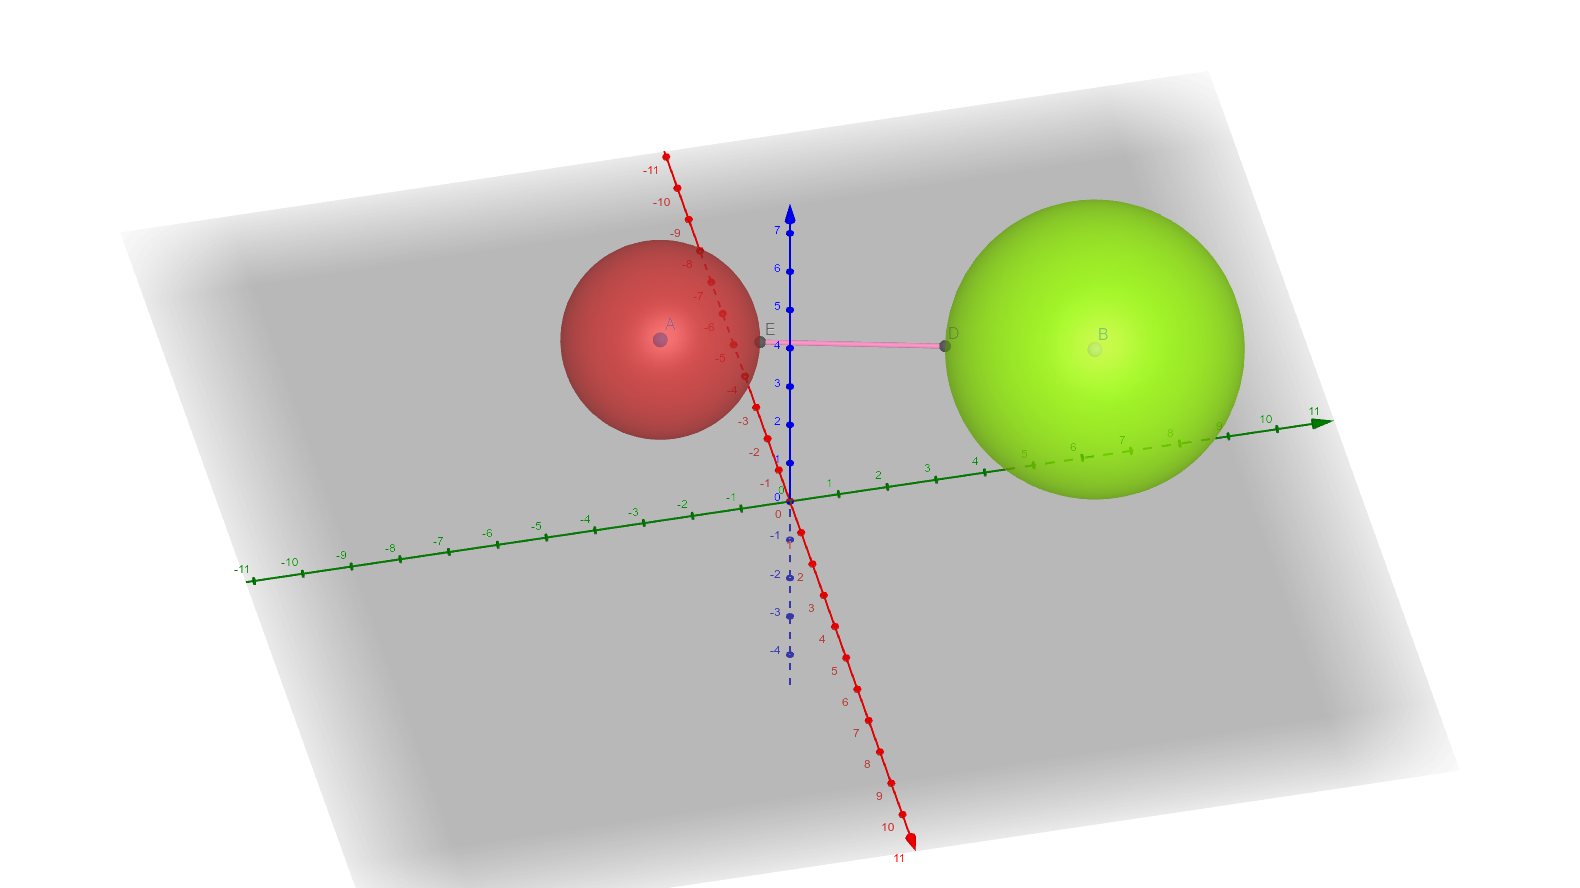
\includegraphics[scale=0.1]{images/sphere-sphere.png}
    \caption{A-DRZ architecture system.}
    \label{fig:sphere_sphere}
\end{figure}

2) Sphere - Capsule:

3) Capsule - Capsule:
\subsection{Collision monitoring} %Sam
\subsection{Potential field} %Sam
\subsection{Controller} %Sam

\section{Experiments}

\subsection{Testing} %Sam
% Not sure on name something to do with implementation
\subsection{ROS} %Brennan
\subsection{Results} %Brennan

\section{Use case}

\subsection{Single arm} %Alan
\subsection{Dual arm} %Alan
\subsection{Self collision} %Alan

\section{Conclusion} %Alan



\addtolength{\textheight}{-12cm}   % This command serves to balance the column lengths
                                  % on the last page of the document manually. It shortens
                                  % the textheight of the last page by a suitable amount.
                                  % This command does not take effect until the next page
                                  % so it should come on the page before the last. Make
                                  % sure that you do not shorten the textheight too much.

%%%%%%%%%%%%%%%%%%%%%%%%%%%%%%%%%%%%%%%%%%%%%%%%%%%%%%%%%%%%%%%%%%%%%%%%%%%%%%%%



%%%%%%%%%%%%%%%%%%%%%%%%%%%%%%%%%%%%%%%%%%%%%%%%%%%%%%%%%%%%%%%%%%%%%%%%%%%%%%%%



%%%%%%%%%%%%%%%%%%%%%%%%%%%%%%%%%%%%%%%%%%%%%%%%%%%%%%%%%%%%%%%%%%%%%%%%%%%%%%%%
\section*{Appendices}

\section*{Acknowledgments}


%%%%%%%%%%%%%%%%%%%%%%%%%%%%%%%%%%%%%%%%%%%%%%%%%%%%%%%%%%%%%%%%%%%%%%%%%%%%%%%%


\begin{thebibliography}{99}

\bibitem{1} H. Hoffmann, P. Pastor, D.-H. Park, and S. Schaal, “Biologically-inspired dynamical systems for movement generation: Automatic real-time goal adaptation and obstacle avoidance,” in 2009 IEEE International Conference on Robotics and Automation, Kobe, May 2009, pp. 2587–2592, doi: 10.1109/ROBOT.2009.5152423.
\bibitem{2} M. Velliste, S. Perel, M. C. Spalding, A. S. Whitford, and A. B. Schwartz, “Cortical control of a prosthetic arm for self-feeding,” Nature, vol. 453, no. 7198, Art. no. 7198, Jun. 2008, doi: 10.1038/nature06996.
\bibitem{3} S. Adee, “Dean Kamen’s ‘Luke Arm’ Prosthesis Readies for Clinical Trials - IEEE Spectrum,” IEEE Spectrum: Technology, Engineering, and Science News, Feb. 01, 2008. https://spectrum.ieee.org/biomedical/bionics/dean-kamens-luke-arm-prosthesis-readies-for-clinical-trials (accessed Jun. 25, 2020).
\bibitem{4} F. Janabi-Sharifi and D. Vinke, “Integration of the artificial potential field approach with simulated annealing for robot path planning,” in Proceedings of 8th IEEE International Symposium on Intelligent Control, Aug. 1993, pp. 536–541, doi: 10.1109/ISIC.1993.397640.
\bibitem{5} O. Khatib, “Real-Time Obstacle Avoidance for Manipulators and Mobile Robots,” The International Journal of Robotics Research, vol. 5, no. 1, pp. 90–98, Mar. 1986, doi: 10.1177/027836498600500106.



\end{thebibliography}


\end{document}
